\documentclass[tikz]{standalone}
\usepackage{amsmath}
\begin{document}
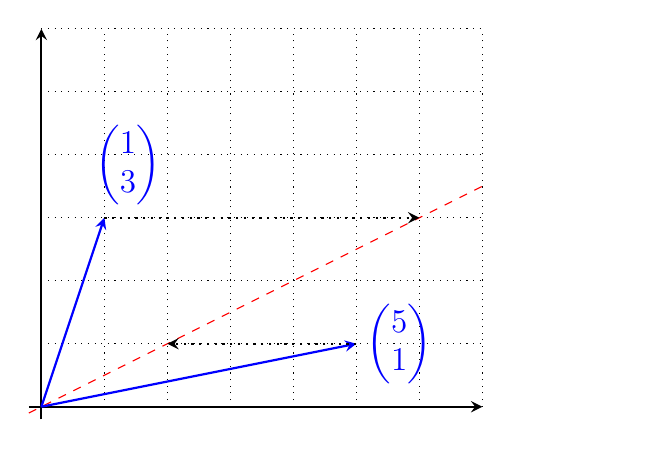
\begin{tikzpicture}[scale=0.8]

% axes
  \draw[thick,>=stealth,->]           (0,-0.2) -- (0,6);
  \draw[thick,>=stealth,->]           (-0.2,0) -- (7,0);

% grid lines
   \draw[step=1.0,black,thin,dotted,xshift=1cm,yshift=1cm] (-1,-1) grid (6,5);

% draw the output line
  \draw[thin,draw=red, dashed] (-0.2,-0.1) -- (7,3.5)  node[right, text=blue, text width=5em] {};

% starting vector blue, transformed vector red
  \draw[thick,>=stealth,->,draw=blue] (0,0) -- (5,1)  node[right, text=blue,  text width=5em] {\large $\mathbf{\begin{pmatrix} 5 \\ 1 \end{pmatrix}}$};
  \draw[thick,>=stealth,->,dotted,draw=black] (5,1) -- (2,1);
  \draw[thick,>=stealth,->,draw=blue] (0,0) -- (1,3)  node[text=blue, label={[xshift=0.3cm, yshift=-0.1cm]\large $\color{blue}{\mathbf{\begin{pmatrix} 1 \\ 3 \end{pmatrix}}}$}] (x2) {};
  \draw[thick,>=stealth,->,dotted,draw=black] (1,3) -- (6,3);

\end{tikzpicture}
\end{document}